\documentclass[a4paper,12pt]{report}

\usepackage{alltt, fancyvrb, url}
\usepackage{graphicx}
\usepackage[utf8]{inputenc}
\usepackage{float}
\usepackage{xcolor}
\usepackage{hyperref}

% Questo commentalo se vuoi scrivere in inglese.
\usepackage[italian]{babel}

\usepackage[italian]{cleveref}

\title{Relazione Temple-Tower per\\``Programmazione ad Oggetti''}

\author{Davide Vignali, Marko Cobo, Mattia Mularoni, Nicolas Montanari}
\date{\today}


\begin{document}

\maketitle

\tableofcontents

\chapter{Analisi}

\section{Descrizione e requisiti}

Il progetto Temple Tower si ispira ai classici dungeon crawler, offrendo un'esperienza di gioco a livelli in cui il giocatore esplora i piani di un dungeon circolare alla ricerca di tesori, affronta nemici e procede al piano successivo, culminando in un epico scontro con un boss finale.
%
La struttura dei livelli, con meccaniche ispirate al gioco \href{https://ring-of-pain.fandom.com/wiki/Ring_of_Pain_Wiki}{Ring of Pain}, garantisce partite sempre diverse.

\subsection*{Requisiti funzionali}
\begin{itemize}
	\item L'area di gioco è circolare ed è composta da diverse caselle contenenti elementi che possono avere effetti positivi o negativi sul giocatore.
	\item Gli elementi di gioco includono tesori (che possono fornire punti esperienza o armi), trappole (che riducono i punti vita) e scale (che permettono al giocatore di salire al piano successivo).
	\item Il giocatore può muoversi liberamente all'interno del livello, combattere contro i nemici e interagire con gli elementi del gioco.
	\item Ogni scontro o attraversamento di una trappola determina la perdita di punti vita; al raggiungimento dello zero, la partita termina e si torna alla schermata iniziale.
    \item La generazione casuale della torre garantisce variabilità e nuove sfide ad ogni partita.
\end{itemize}

\subsection*{Requisiti non funzionali}
\begin{itemize}
	\item All'ultimo piano il giocatore affronterà un boss finale dotato di comportamenti unici e di una difficoltà superiore rispetto ai nemici ordinari.
	\item La difficoltà si adatta dinamicamente in base al percorso del giocatore.
	\item È prevista una musica di sottofondo e feedback sonori per ogni azione significativa.
	\item Sono disponibili diverse tipologie di armi, la cui efficacia varia in base al tipo di nemico affrontato.
\end{itemize}

\section{Modello del Dominio}
\textbf{Temple Tower} verrà rappresentato da una torre composta da un certo numero di piani (\textit{Floor}), 
%
ciascuno dei quali ospiterà stanze interconnesse. Ogni stanza potrà contenere una trappola, un nemico, un tesoro e ospitare il giocatore.

\begin{itemize}
    \item \textbf{Trappole}: infliggono danni al giocatore.
    \item \textbf{Nemici}: attaccano il giocatore in combattimenti a turni.
    \item \textbf{Tesori}: forniscono punti vita, nuove armi oppure possono essere una trappola.
\end{itemize}
%
Il giocatore potrà utilizzare armi per affrontare i nemici. Poiché gli attacchi avvengono a turni, 
%
è fondamentale bilanciare le statistiche per evitare vittorie "matematiche" dovute a disparità nell'efficacia delle armi. 
%
Il giocatore e i nemici disporranno di diverse tipologie di mosse d'attacco e armi, che possono variare in potenza ed effetto.
%
Dopo aver esplorato le stanze di un piano, il giocatore potrà utilizzare le scale per salire al piano successivo della torre. 
%
Durante la partita, sia il giocatore sia i nemici disporranno di barre di stato: \textbf{vita}.
%
\begin{itemize}
    \item \textbf{Barra della vita}: si riduce subendo danni da nemici o trappole. Quando raggiunge lo zero, la partita termina e si ricomincia dall'inizio.
\end{itemize}
%
All’ultimo piano, il giocatore affronterà il \textbf{boss finale}, un nemico più forte dotato di mosse d'attacco avanzate e particolari rispetto ai nemici ordinari.
%
Per arricchire l’esperienza, sarà presente un sottofondo musicale durante tutto il gioco.
%
\begin{figure}[H]
	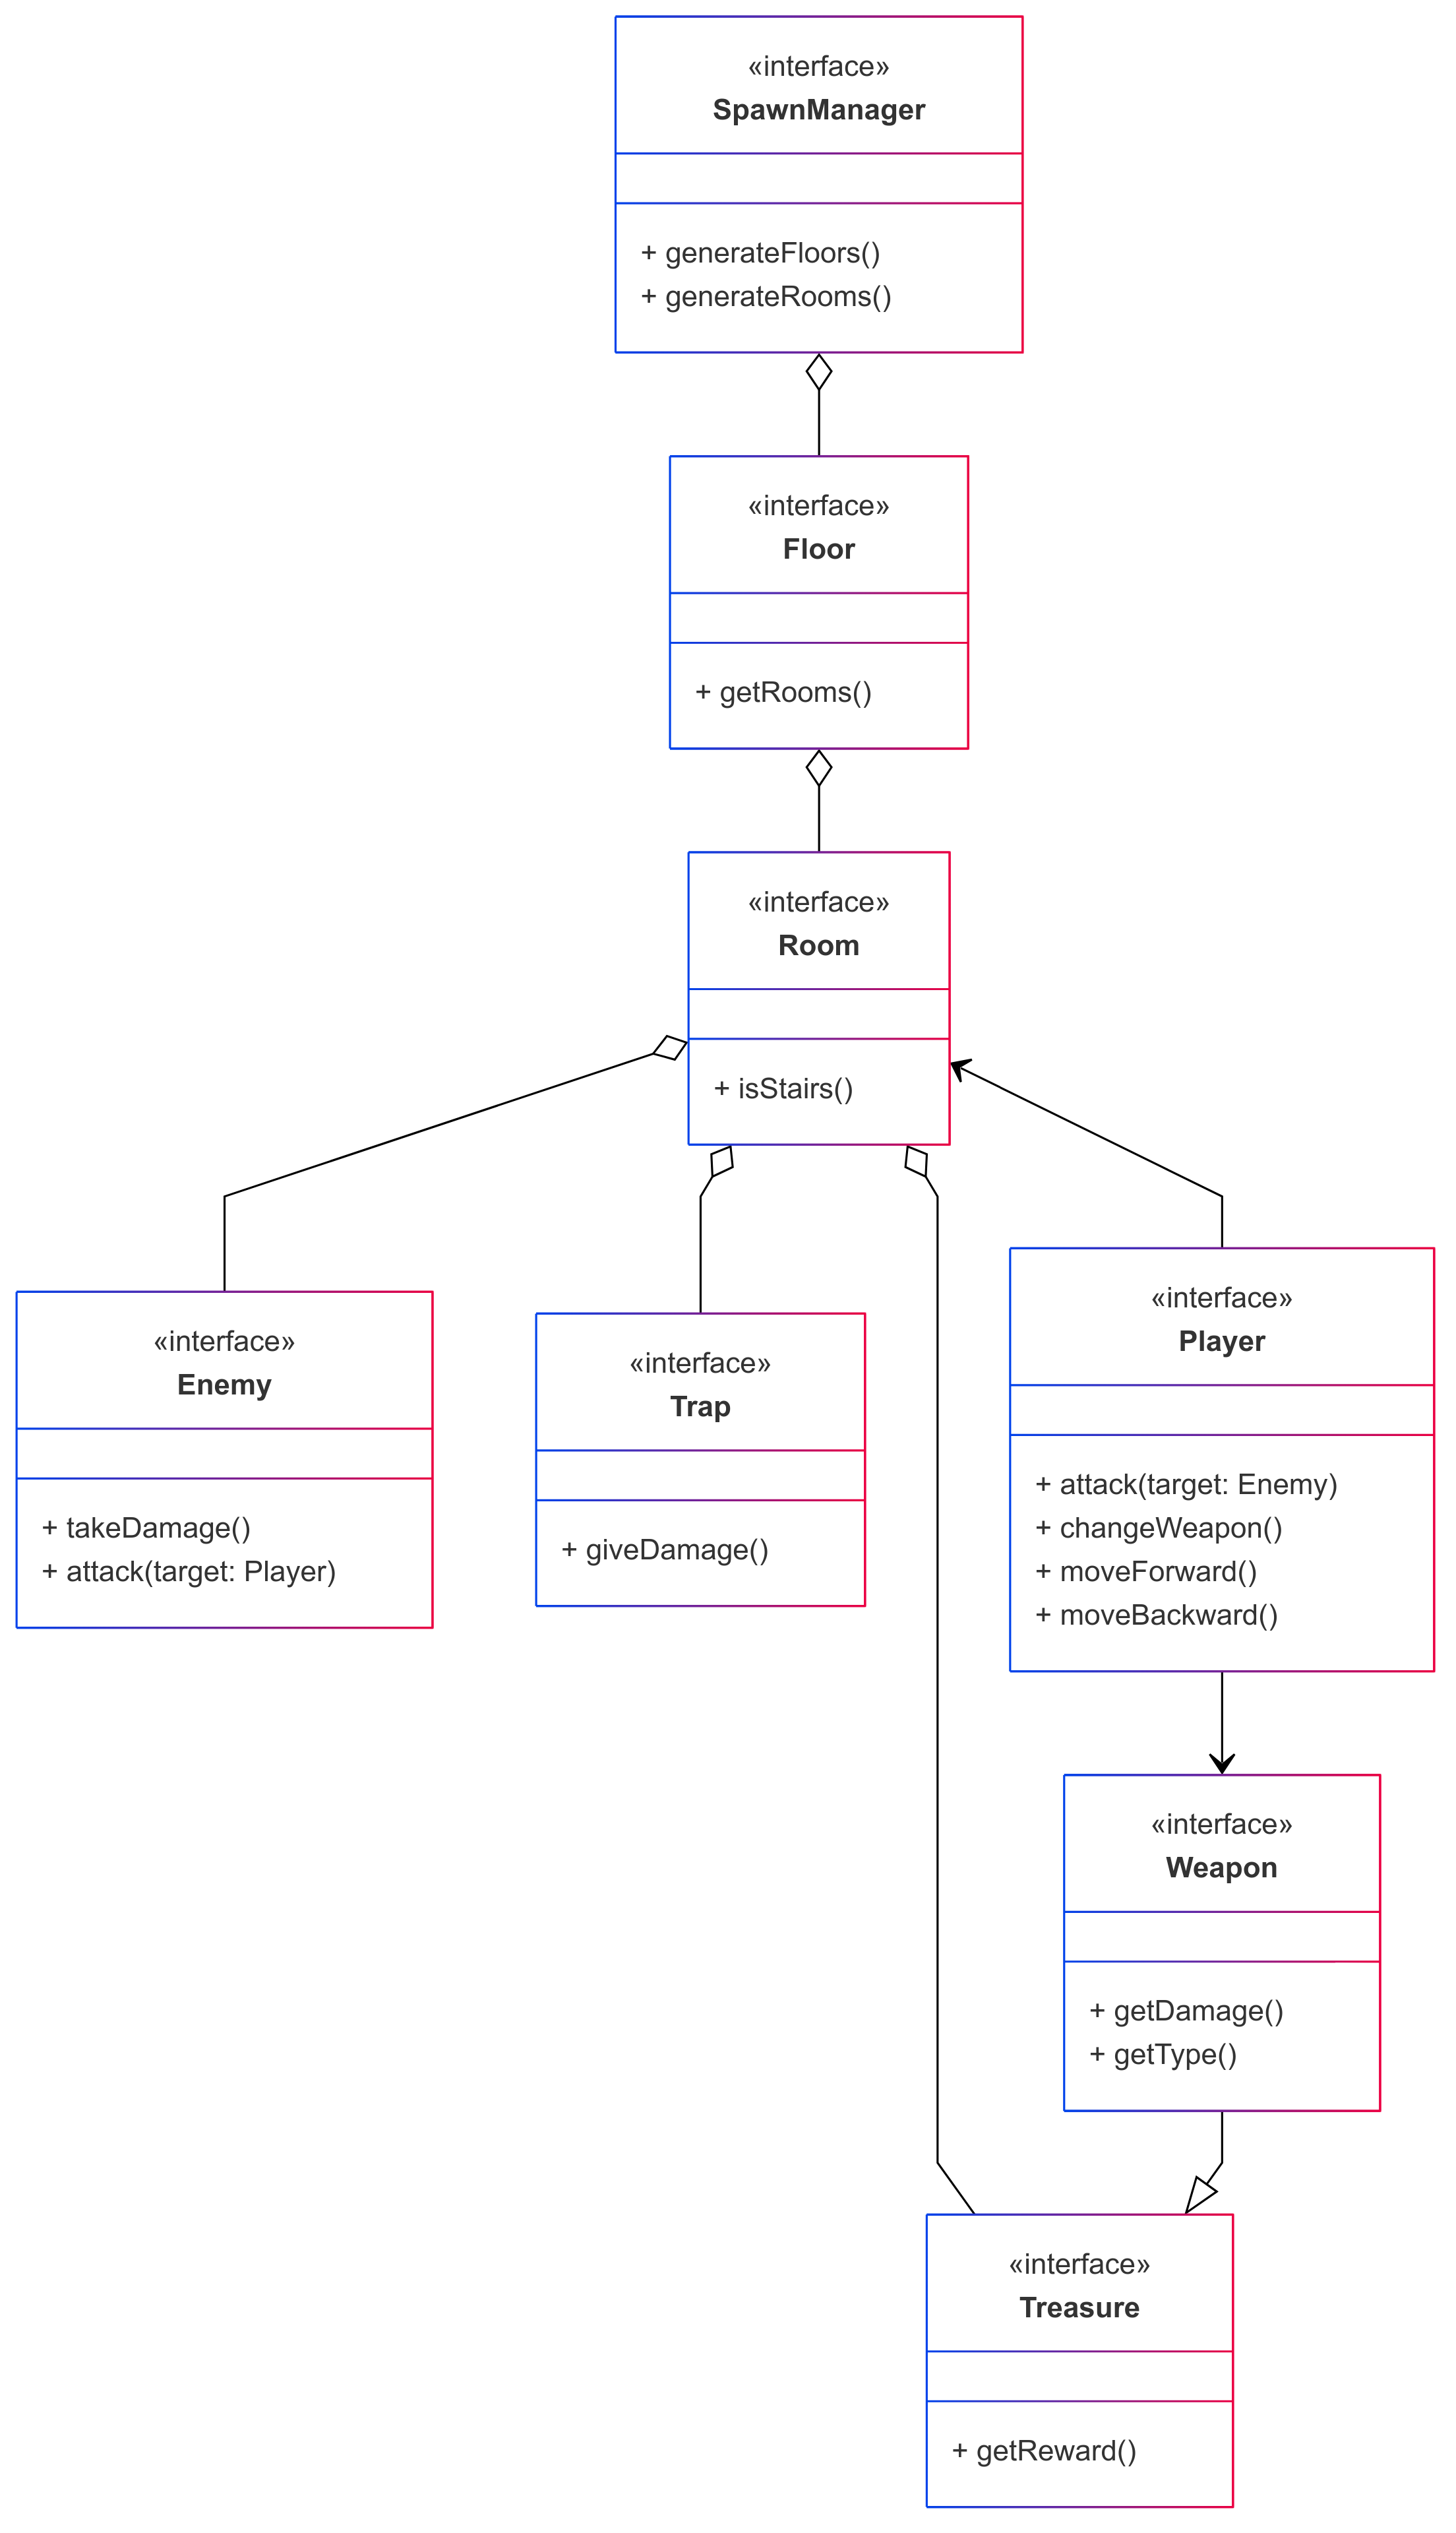
\includegraphics[scale=0.15]{img/analisys.png}
\end{figure}

\chapter{Design}

\section{Architettura}

L'architettura del gioco \textbf{Temple Tower} segue il pattern architetturale \textbf{Model-View-Controller (MVC)} per garantire una chiara separazione delle responsabilità tra la logica di business, la presentazione e la gestione degli eventi.

\subsection*{Composizione del Pattern MVC}
\begin{itemize}
    \item \textbf{Model}: 
    \begin{itemize}
        \item Rappresenta la logica principale del gioco e include classi come \texttt{Tower}, \texttt{Floor}, \texttt{RoomBehavior}, \texttt{Player} e i vari tipi di stanze (\texttt{EnemyRoom}, \texttt{TreasureRoom}, \texttt{StairsRoom}) che implementano il pattern Strategy.
        \item Questo approccio consente di definire comportamenti specifici per ogni tipologia di stanza in modo modulare, rendendo semplice l'aggiunta di nuovi tipi di stanze senza modificare il codice esistente.
        \item La logica di gioco, come il movimento del giocatore o gli effetti delle interazioni con nemici, trappole o tesori, è interamente contenuta nel model.
    \end{itemize}

    \item \textbf{View}: 
    \begin{itemize}
        \item La view è gestita da un \texttt{SceneManager} che, mediante l'implementazione di un pattern Factory, si occupa del cambio della vista in base alla situazione attuale.
        \item Grazie al manager è possibile decentralizzare le responsabilità della view in diverse classi, ciascuna responsabile della gestione degli eventi della propria interfaccia.
    \end{itemize}

    \item \textbf{Controller}: 
    \begin{itemize}
        \item La classe \texttt{GameController} funge da intermediario tra il modello e la vista, orchestrando il flusso degli eventi nel gioco.
        \item Gestisce le azioni dell'utente, permettendo al giocatore di muoversi tra le stanze (metodo \texttt{changeRoom}) o salire al piano successivo (metodo \texttt{gotoNextFloor}), e si occupa inoltre di iniziare e terminare il gioco.
    \end{itemize}
\end{itemize} 

\subsection*{Scalabilità e Manutenibilità}
Grazie all'uso combinato dei pattern MVC e Strategy:
\begin{itemize}
    \item \textbf{Aggiunta di nuove stanze}: È possibile introdurre nuove tipologie di stanze semplicemente aggiungendo nuove implementazioni dell'interfaccia \texttt{RoomBehavior}, senza modificare altre parti del codice.
    \item \textbf{Separazione delle responsabilità}: La gestione della logica di gioco, della presentazione grafica e delle interazioni dell'utente è ben separata, favorendo la manutenibilità e la possibilità di modificare singole componenti senza influenzare l'intero sistema.
\end{itemize}

Questa architettura rende il sistema flessibile, modulare e facilmente estensibile, adattandosi alle necessità di futuri miglioramenti o aggiunte.
%
\begin{figure}[H]
	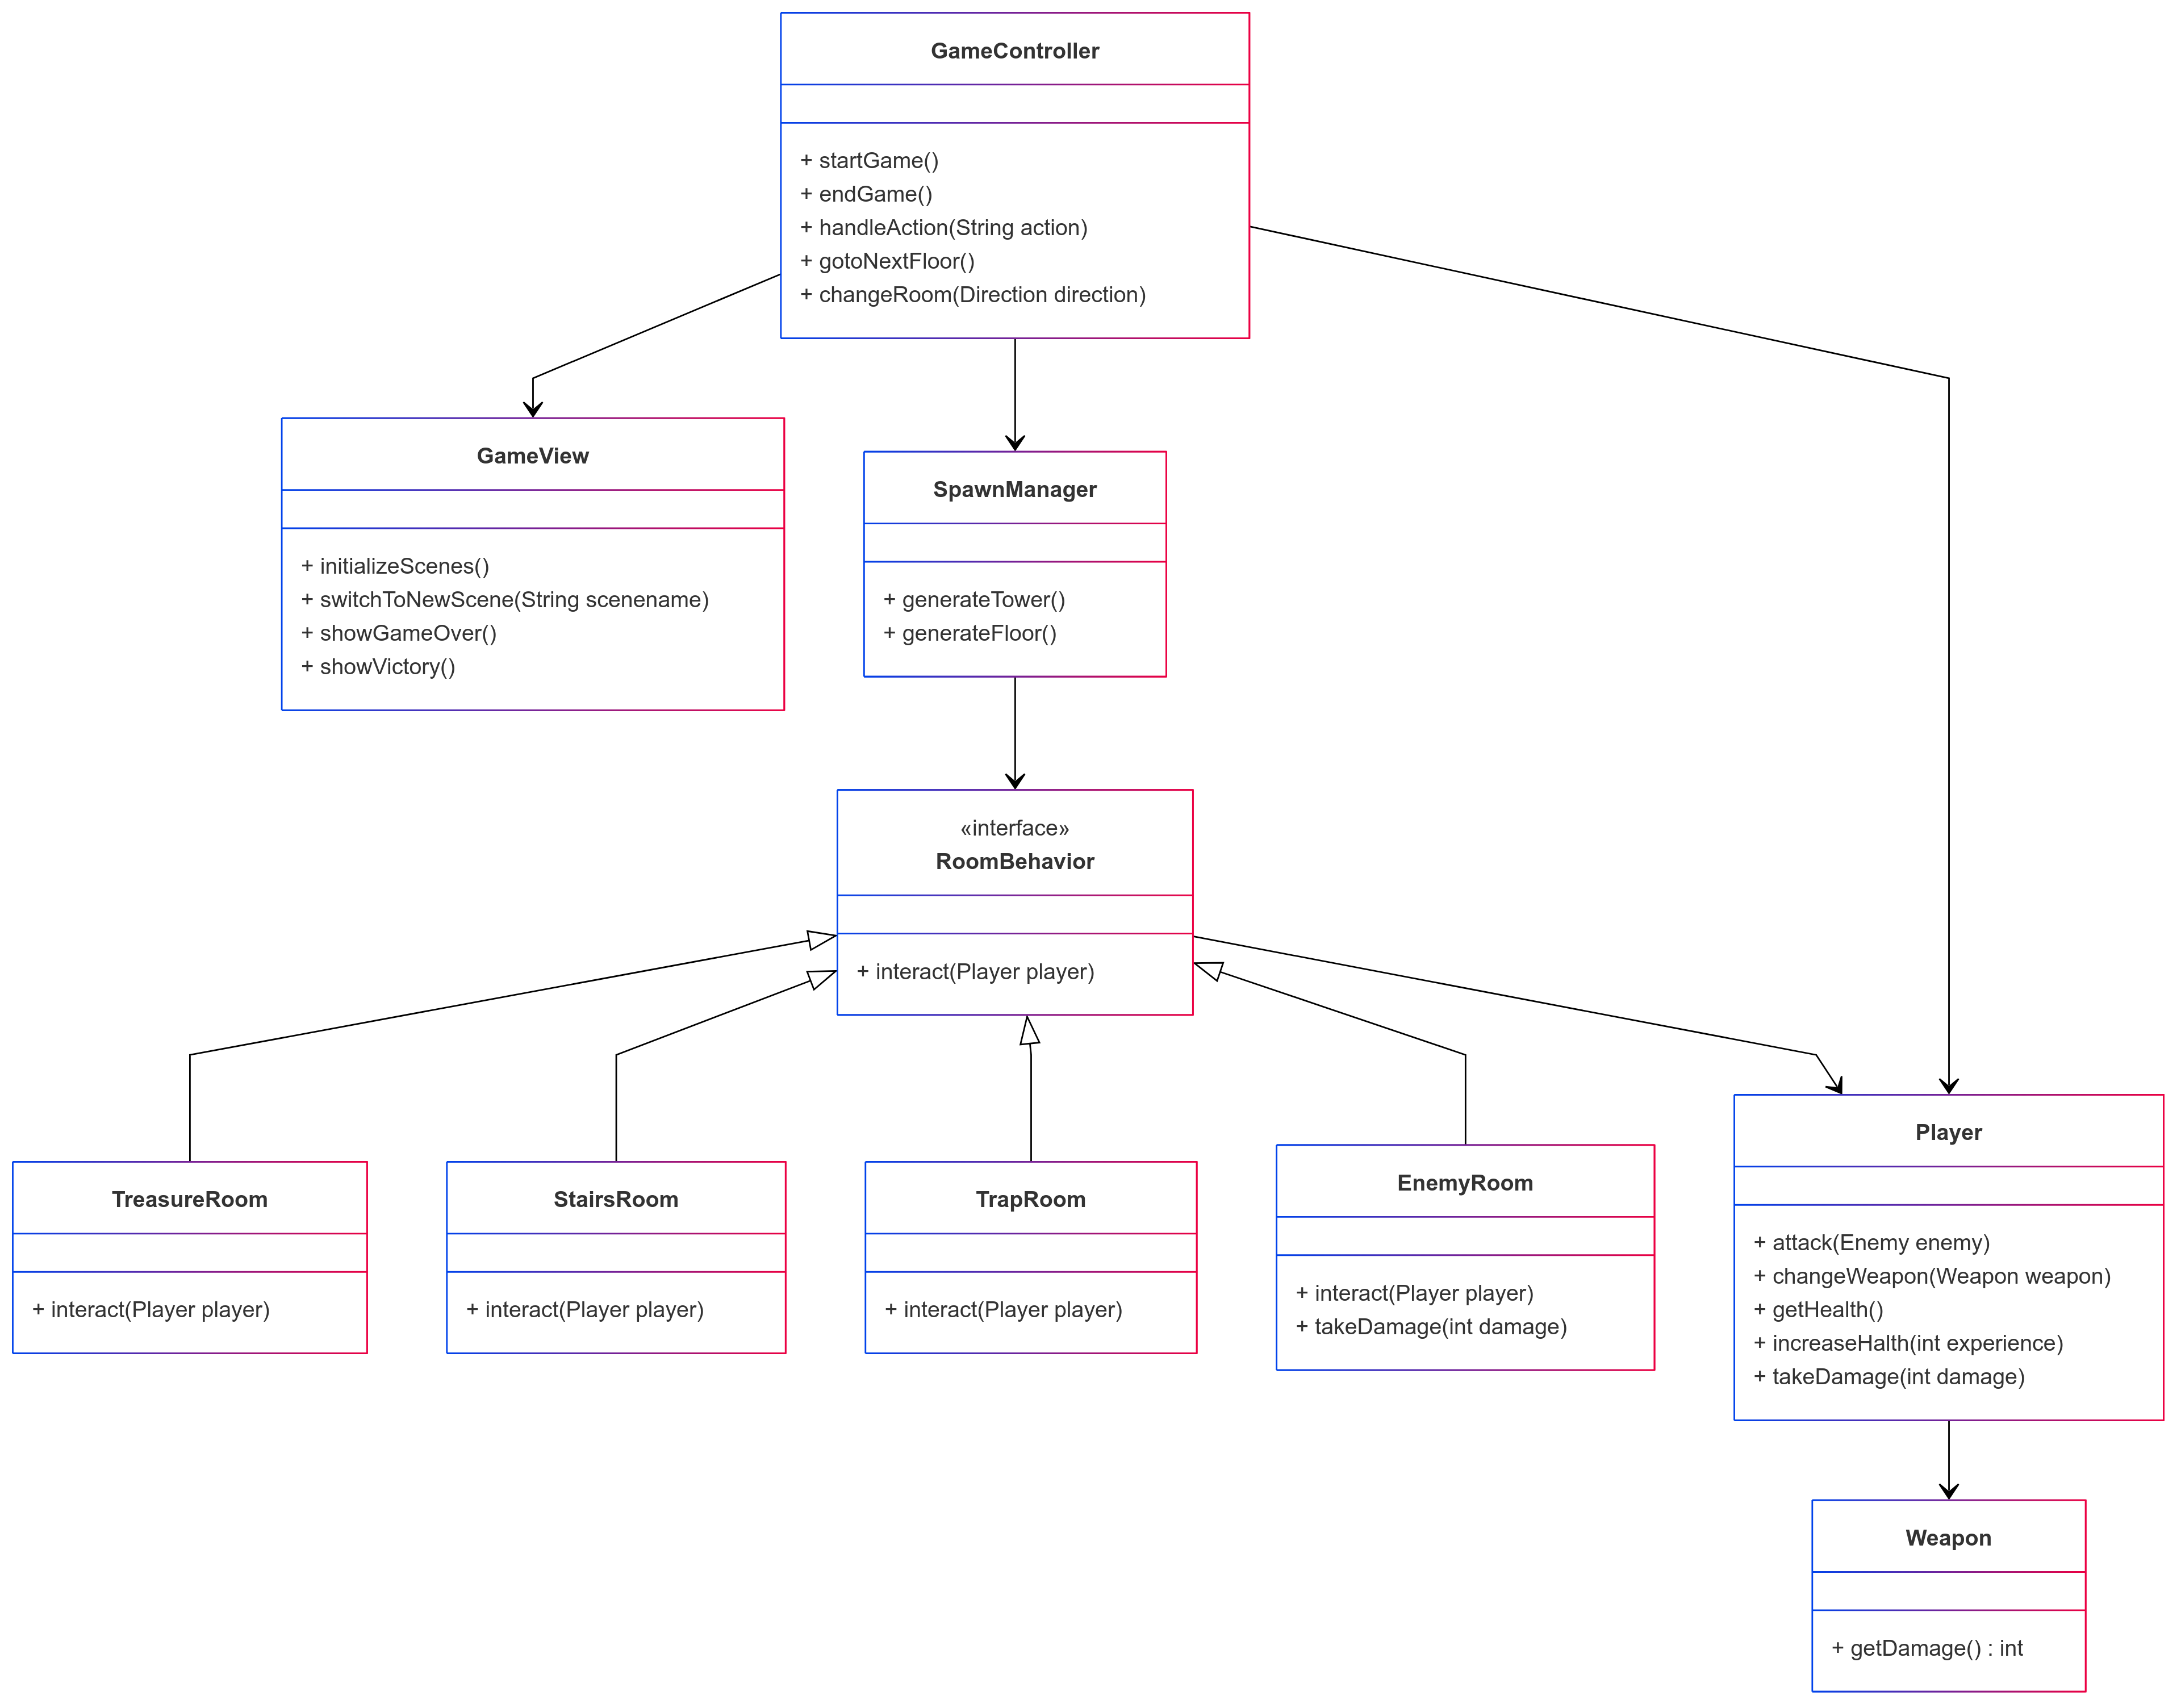
\includegraphics[scale=0.12]{img/design.png}
\end{figure}

\section{Design dettagliato}
\subsection{Cobo}
\subsubsection{Sistema di Gestione Audio}
Il sistema richiede una gestione per la riproduzione della musica di sottofondo, le cui funzionalità principali sono:
\begin{itemize}
    \item Gestione del volume;
    \item Controllo dello stato di riproduzione della musica;
    \item Corretto caricamento e gestione delle risorse audio;
    \item Mantenimento di una netta separazione tra logica, controllo e view.
\end{itemize}

\textbf{Architettura MVC}\newline
La soluzione proposta implementa un pattern Model-View-Controller (MVC) con le seguenti componenti:
\begin{itemize}
    \item \textbf{Model (MusicModel)}: Mantiene informazioni sul volume e sullo stato della riproduzione, gestisce il ciclo di vita del clip audio e lo stato interno del sistema.
    \item \textbf{Controller (MusicController)}: Gestisce le operazioni sulla riproduzione musicale, fungendo da intermediario tra View e Model.
    \item \textbf{View}: Richiama i metodi del controller per gestire la riproduzione.
\end{itemize}

\textbf{Vantaggi e svantaggi}\newline
\textbf{Pro}: Separazione delle responsabilità – il MusicModel si occupa dei dettagli tecnici mentre il MusicController gestisce il flusso principale.

\textbf{Contro}: Richiede una buona coordinazione tra le classi.

\textbf{Diagramma UML}\newline
\begin{figure}[h]
    \centering 
    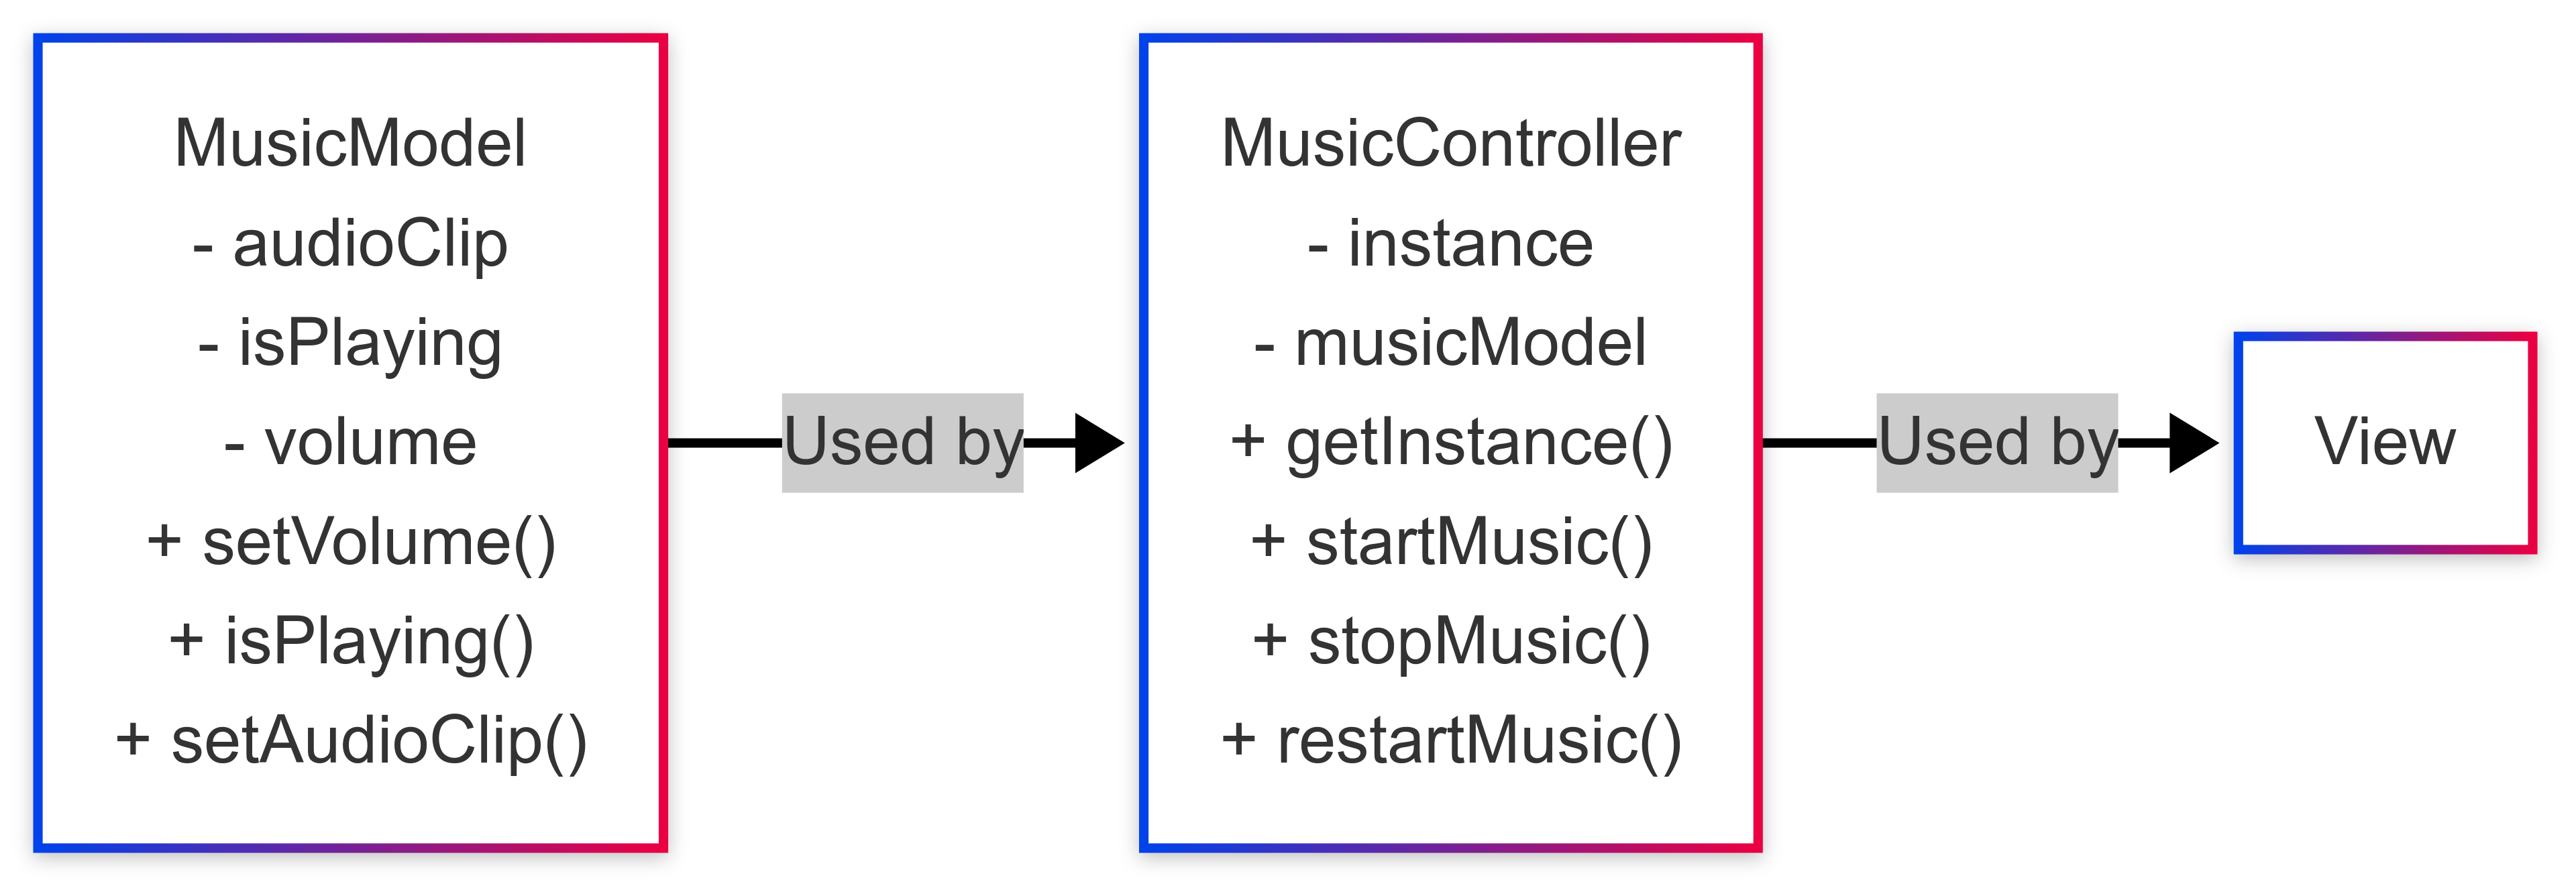
\includegraphics[width=0.8\textwidth]{img/uml_diagram.png}
    \caption{Diagramma UML del sistema di gestione audio}
    \label{fig:uml}
\end{figure}

\subsubsection{Pattern Singleton}
Il pattern Singleton è stato utilizzato nella classe \texttt{MusicController} per garantire l'unicità dell'istanza del controller musicale durante l'esecuzione dell'applicazione, evitando conflitti e garantendo un punto d'accesso globale alla gestione audio.

\subsubsection{Metodo Template: getInstance()}
\textbf{Motivazione}: Assicura l'unicità dell'istanza di \texttt{MusicController}, facilitando la gestione centralizzata della riproduzione musicale. Il pattern Singleton è stato implementato correttamente, considerando che la gestione centralizzata richiede una sola istanza.

\subsection{Montanari}
\subsubsection{Gestione dei Popup tramite Factory Method}

\textbf{Problema}\newline
Nel gioco esistono diversi tipi di finestre di dialogo (popup) per situazioni come la raccolta di un'arma o il guadagno di esperienza. La creazione manuale di questi popup in ogni punto del codice porta a duplicazioni e a una minore manutenibilità. Inoltre, l'assenza di un'adeguata astrazione comporterebbe la necessità di riscrivere la struttura per ogni nuovo popup, aumentando il rischio di incoerenze.
  
\textbf{Soluzione}\newline
È stato adottato il Factory Method per delegare la creazione dei popup a una classe centralizzata (\texttt{DialogFactory}). Questa classe definisce il metodo \texttt{createDialog} che, in base al tipo di popup richiesto, restituisce un oggetto \texttt{Dialog} con il contenuto e il comportamento appropriati.

Questa soluzione offre diversi vantaggi:
\begin{itemize}
\item \textbf{Miglior riuso del codice}: la logica di costruzione dei popup è centralizzata e riutilizzabile.
\item \textbf{Maggiore manutenibilità}: per aggiungere nuovi tipi di popup, basta estendere il metodo \texttt{createDialog} senza modificare il codice esistente.
\item \textbf{Maggiore coerenza}: tutti i popup adottano uno stile uniforme e una gestione standardizzata degli eventi.
\end{itemize}

Un’alternativa considerata era l’uso di una classe \texttt{DialogUtil} con metodi statici per ogni tipo di popup, ma tale approccio avrebbe reso più difficile l'estensione senza modifiche dirette, violando il principio Open/Closed.

\textbf{Schema UML}\newline
\begin{figure}[H]
	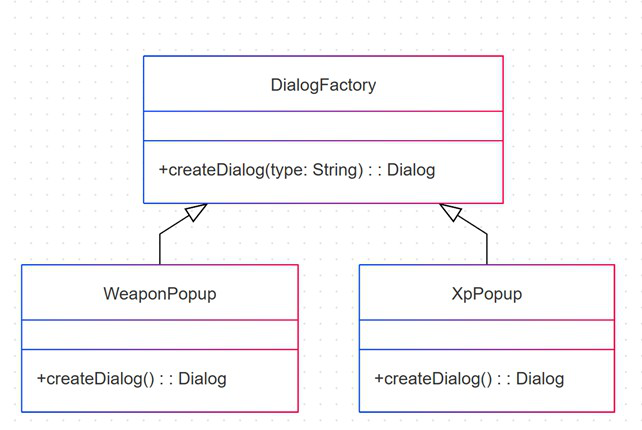
\includegraphics[scale=0.8]{img/montanariDialog.png}
\end{figure}

\textbf{Applicazione del Pattern Factory Method}\newline
\begin{itemize}
\item \texttt{DialogFactory} è la classe che espone il metodo \texttt{createDialog}, delegando la creazione alle sottoclassi specifiche.
\item \texttt{WeaponPopup} e \texttt{XpPopup} sono le sottoclassi che sovrascrivono il metodo factory per fornire l’implementazione specifica.
\item Il codice client utilizza \texttt{DialogFactory.createDialog()} per ottenere il popup corretto senza dover conoscere i dettagli della sua implementazione.
\end{itemize}

Questa implementazione migliora la separazione delle responsabilità e facilita l’aggiunta di nuovi tipi di popup in futuro.

\subsubsection{Gestione della Sincronizzazione tra Attacco, Punti Vita e UI}

\textbf{Problema}\newline
Nella gestione della scena di combattimento è necessario sincronizzare correttamente l'attacco del giocatore, la riduzione dei punti vita dell'avversario e l'aggiornamento dell'interfaccia utente (UI). Una gestione errata potrebbe causare ritardi o incoerenze visive, impattando negativamente il gameplay.
  
\textbf{Soluzione}\newline
La soluzione prevede una gestione sequenziale delle azioni tramite:
\begin{itemize}
    \item \textbf{Animazioni} (\texttt{Timeline}) per gestire i movimenti visivi;
    \item \textbf{Ritardi programmati} (\texttt{PauseTransition}) per sincronizzare le azioni;
    \item \textbf{Aggiornamenti della UI} (\texttt{Platform.runLater}) per eseguire modifiche nel thread principale in modo sicuro.
\end{itemize}

Il flusso esecutivo prevede:
\begin{enumerate}
    \item Esecuzione dell’attacco tramite animazione (ad esempio, una fiamma o un movimento in avanti del giocatore).
    \item Al termine dell’animazione, applicazione del danno riducendo i punti vita dell’avversario.
    \item Aggiornamento della UI, modificando la barra della salute (\texttt{ProgressBar}) e il valore numerico degli HP.
    \item Se il nemico è ancora in vita, attivazione di un ritardo tramite \texttt{PauseTransition} per simulare il tempo di reazione.
    \item Esecuzione del contrattacco nemico con conseguente aggiornamento della UI.
    \item Verifica dello stato del combattimento:
    \item In caso di vittoria del giocatore, il pulsante d'attacco viene disabilitato e la salute ripristinata.
    \item In caso di sconfitta, viene mostrato un popup che reindirizza al menu principale.
\end{enumerate}

\textbf{Schema UML}\newline
\begin{figure}[H]
	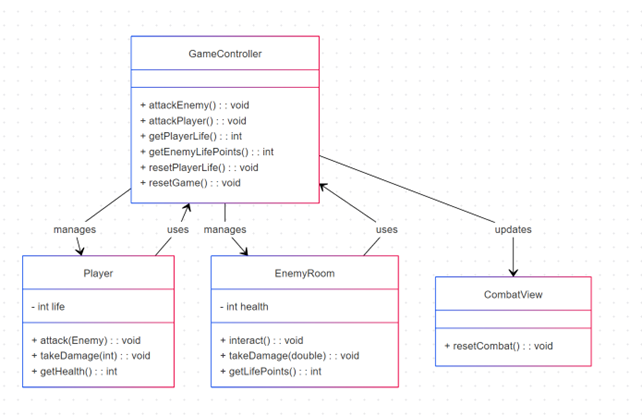
\includegraphics[scale=0.9]{img/montanariPlatform.png}
\end{figure}

\textbf{Benefici ottenuti}\newline
Questa soluzione garantisce una transizione fluida tra attacco, difesa e aggiornamento della UI, prevenendo problemi di desincronizzazione. L’uso di \texttt{Platform.runLater} assicura aggiornamenti sicuri nel thread principale di JavaFX, migliorando la responsività dell'applicazione. Inoltre, le pause controllate migliorano il feedback visivo per il giocatore.

\subsection{Vignali}

\subsubsection{Modular Game Data Loading and Tower Configuration}

\paragraph{Problema} Il sistema deve caricare e gestire dati di gioco da file JSON in modo flessibile, consentendo l'uso sia di torri predefinite sia di mod create dagli utenti. I dati devono essere validati e supportare riferimenti relativi tra file.

\paragraph{Soluzione} Sono stati valutati due approcci:
\begin{enumerate}
    \item Un sistema di caricamento decentralizzato in cui ogni componente gestisce i propri dati;
    \item Un gestore centralizzato che coordina l'intero caricamento.
\end{enumerate}
È stata scelta la seconda opzione, implementando GameDataManagerImpl come Singleton per garantire un punto d'accesso unico. Pur considerando l'uso della Dependency Injection, la natura globale dei dati e la necessità di mantenerli coerenti hanno reso il Singleton l'opzione migliore.

Il sistema utilizza record immutabili (FloorData, Enemy, Weapon) e custom deserializer GSON per garantire type-safety e validazione durante il caricamento. Questa soluzione separa nettamente i dati dalla logica, agevolando l'estensione del sistema con nuove mod.

Schema UML:
\begin{figure}[H]
	\centering
	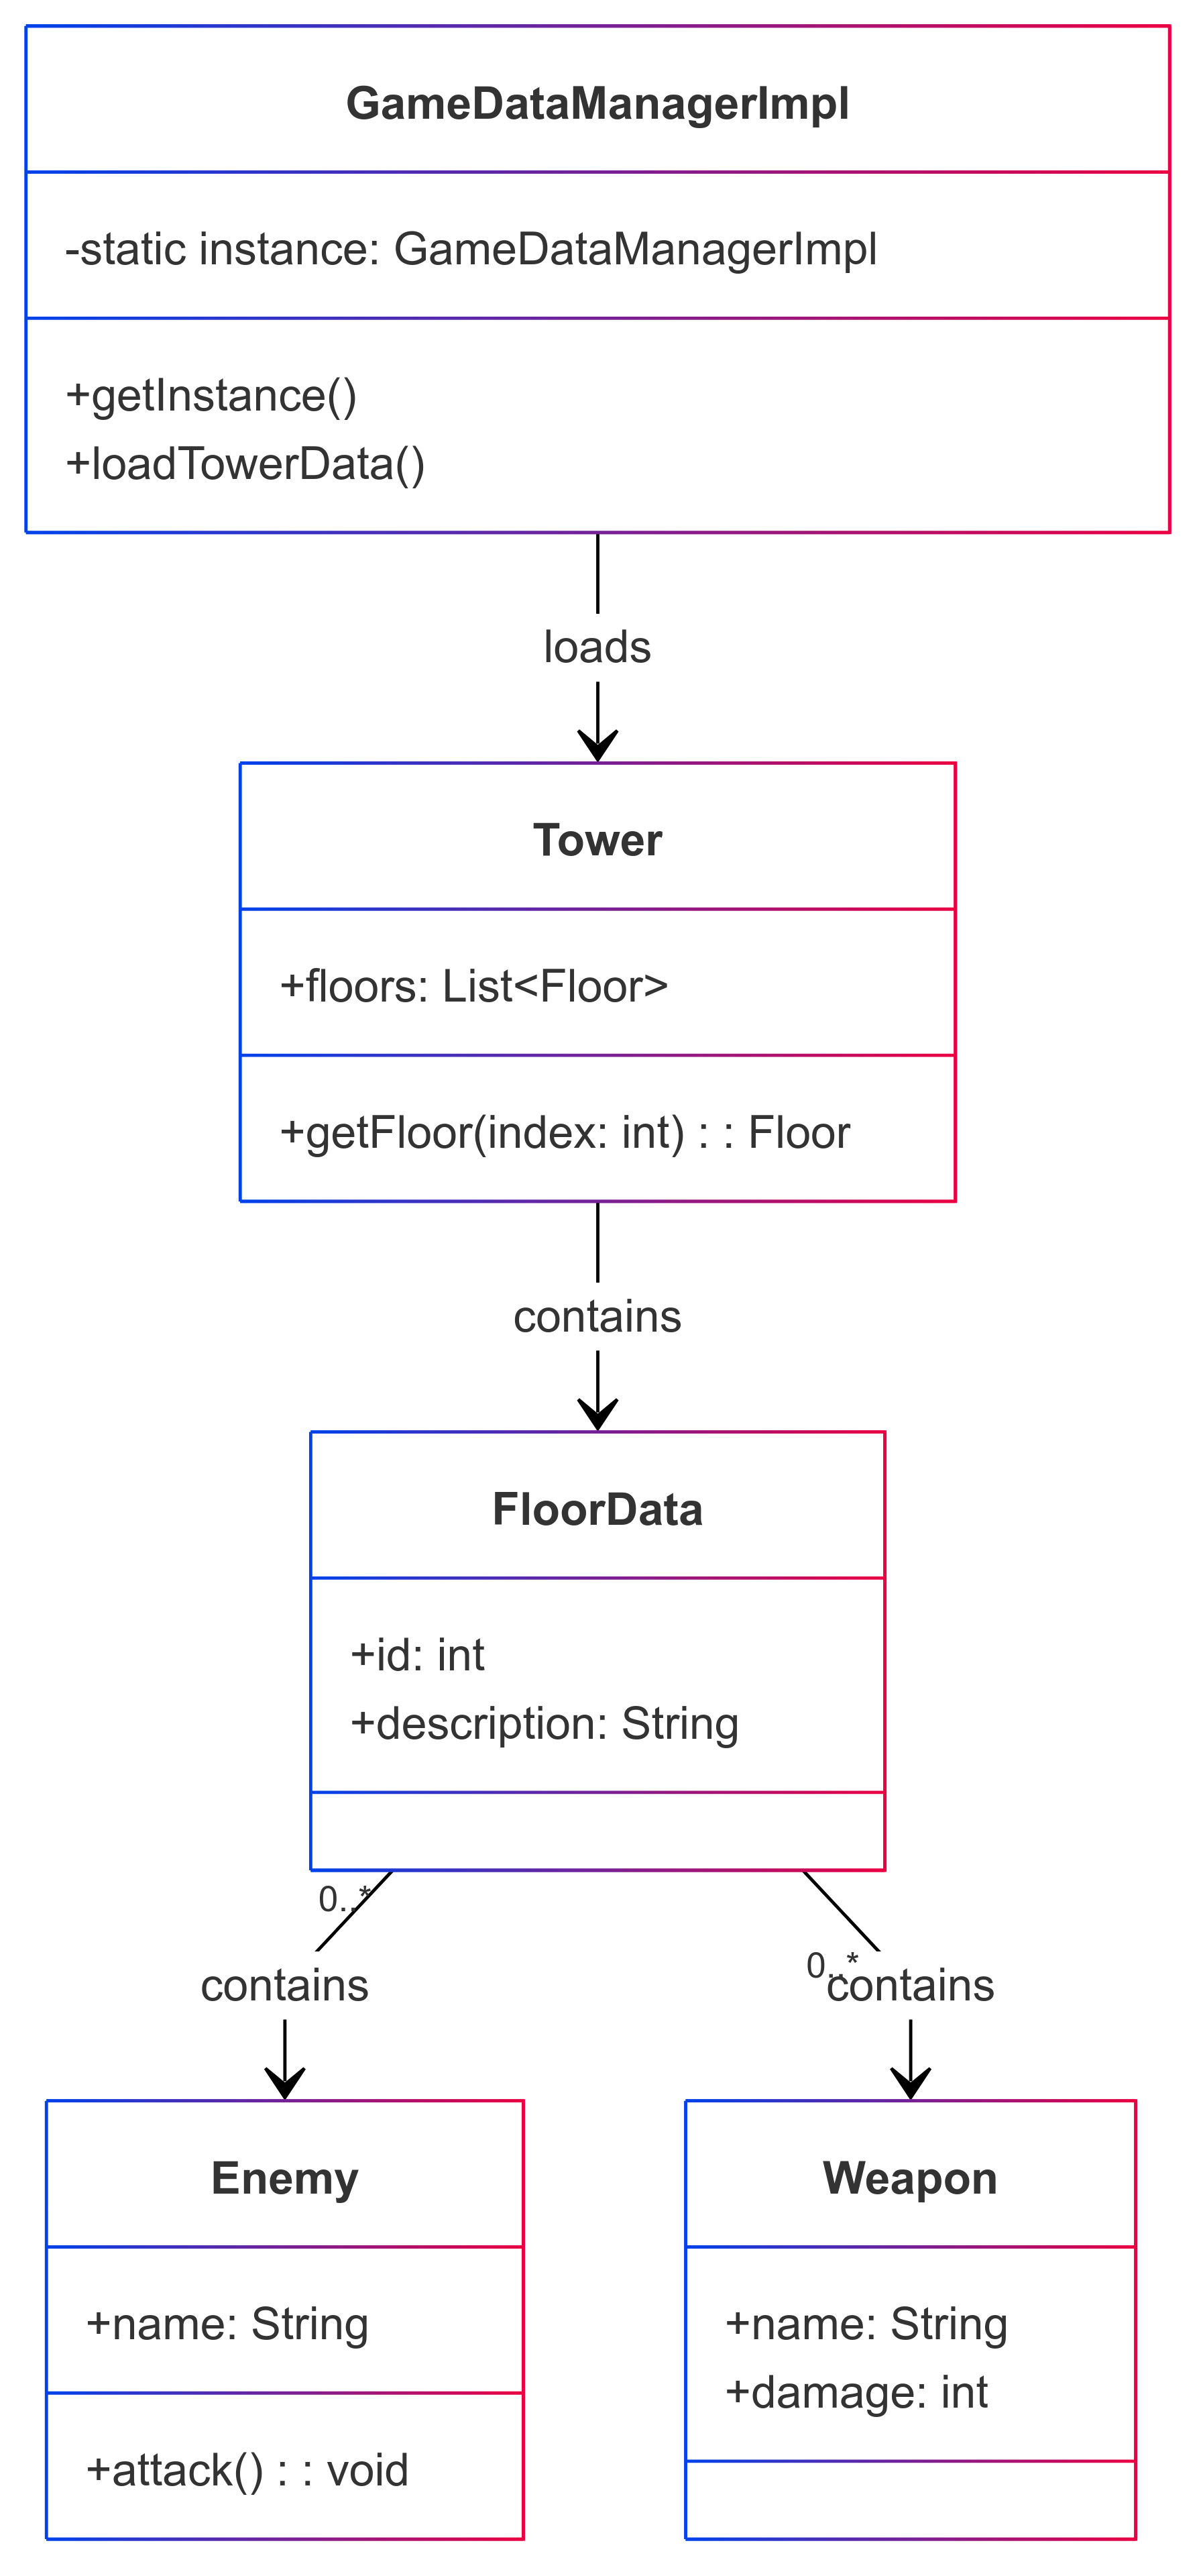
\includegraphics[scale=0.08]{img/GameDataManagerUML.png}
	\caption{GameDataManagerImpl as Singleton and its relations.}
\end{figure}

\subsubsection{Sistema di Modding}

\paragraph{Problema} Il gioco deve permettere agli utenti di creare e importare torri personalizzate (mod) da cartelle o file ZIP, gestendo validazione, conflitti di nomi e isolamento tra mod.

\paragraph{Soluzione} Sono state considerate due architetture:
\begin{enumerate}
    \item Un sistema event-based con chiamate asincrone per l'importazione;
    \item Un'architettura MVC con pattern Observer per la sincronizzazione della UI.
\end{enumerate}
È stata scelta la seconda, che offre una separazione più chiara delle responsabilità e una gestione dello stato più prevedibile. Il pattern Observer è preferito rispetto ai callback per la facilità di estensione senza modifiche al codice esistente.

È stato inoltre implementato il pattern Strategy per supportare nuovi formati di mod, oltre a ZIP e cartelle.

Schema UML:
\begin{figure}[H]
	\centering
	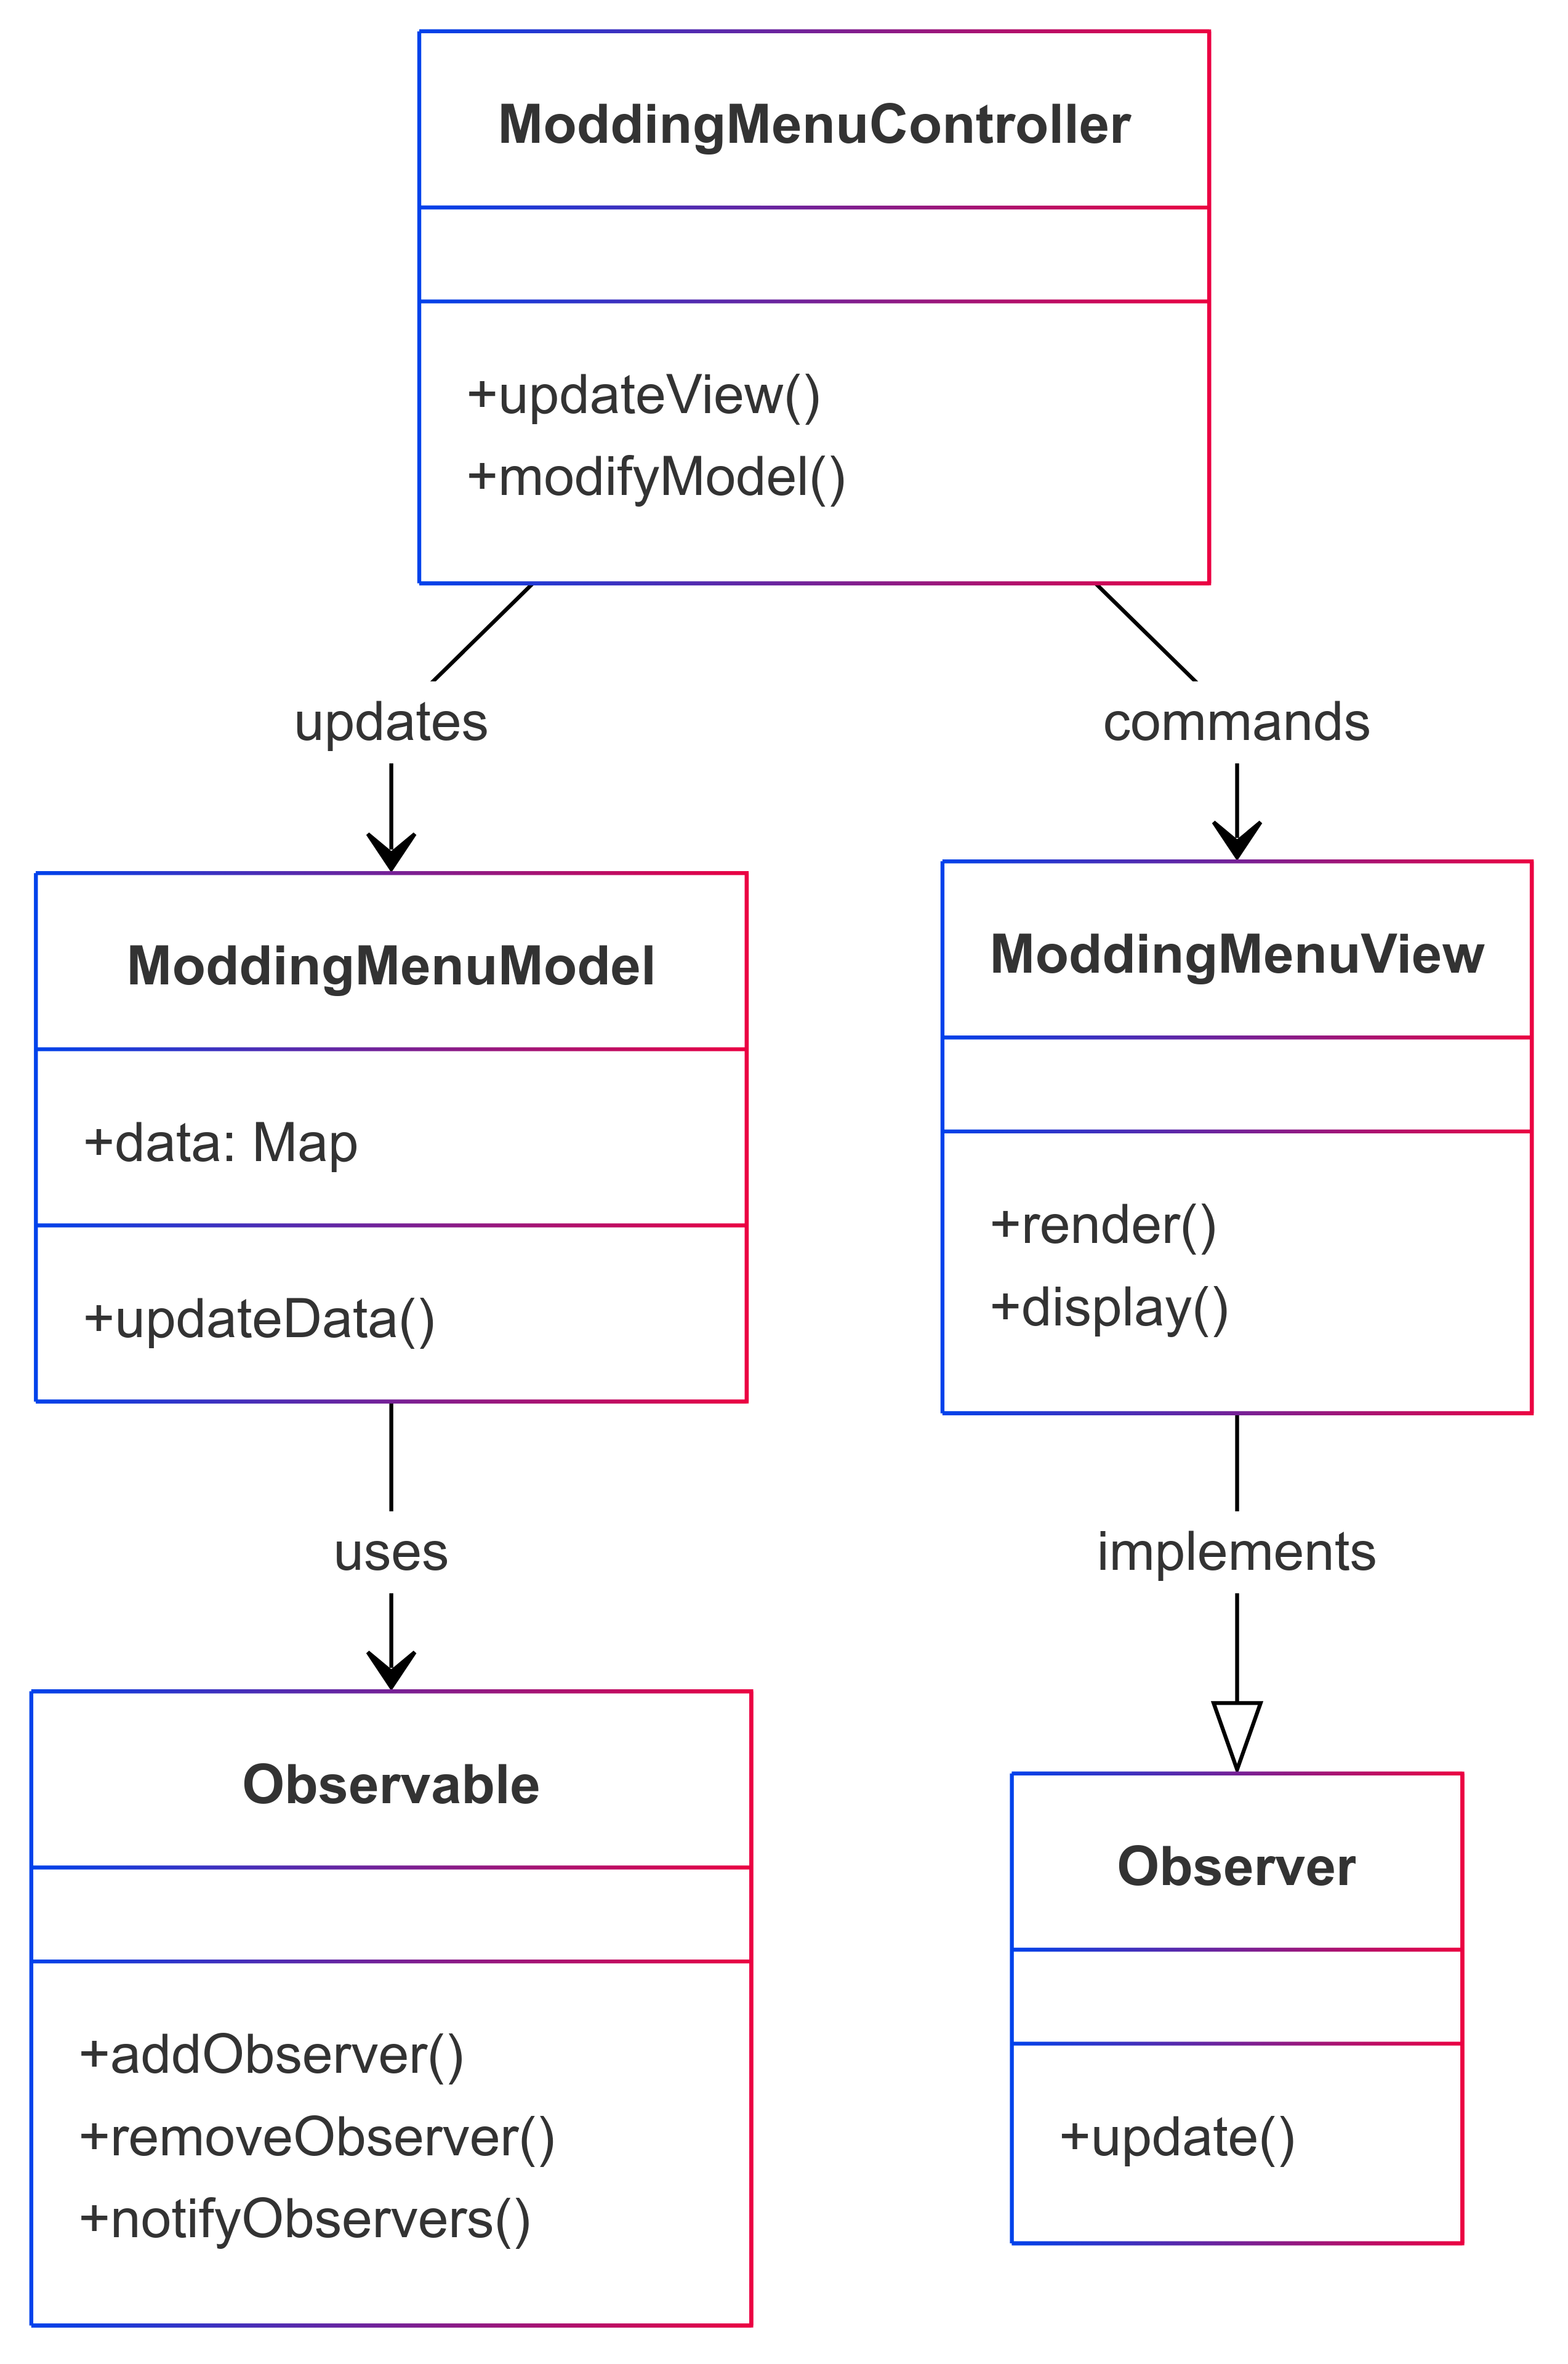
\includegraphics[scale=0.08]{img/ModdingMenuUML.png}
	\caption{Modding Menu UML: MVC and Observer pattern overview.}
\end{figure}

\subsubsection{Gestione dello Spawn System}

\paragraph{Problema} Il sistema deve generare contenuti procedurali bilanciati, rispettando vincoli di livello e configurazioni di spawn.

\paragraph{Soluzione} Sono stati valutati due approcci:
\begin{enumerate}
	\item Generazione puramente casuale con post-validazione;
	\item Sistema template-based con strategie di generazione.
\end{enumerate}
È stato scelto il secondo approccio, implementando un Template Method in SpawnManagerImpl che standardizza il processo di generazione, permettendo variazioni nel comportamento specifico. Il metodo template si articola in tre fasi:
\begin{enumerate}
	\item Selezione del tipo di piano (template method);
	\item Generazione delle stanze (hook method);
	\item Popolamento delle stanze (hook method).
\end{enumerate}

\subsection{Mularoni}

\subsubsection{Cambio vista}

\begin{figure}[H]
\centering{}
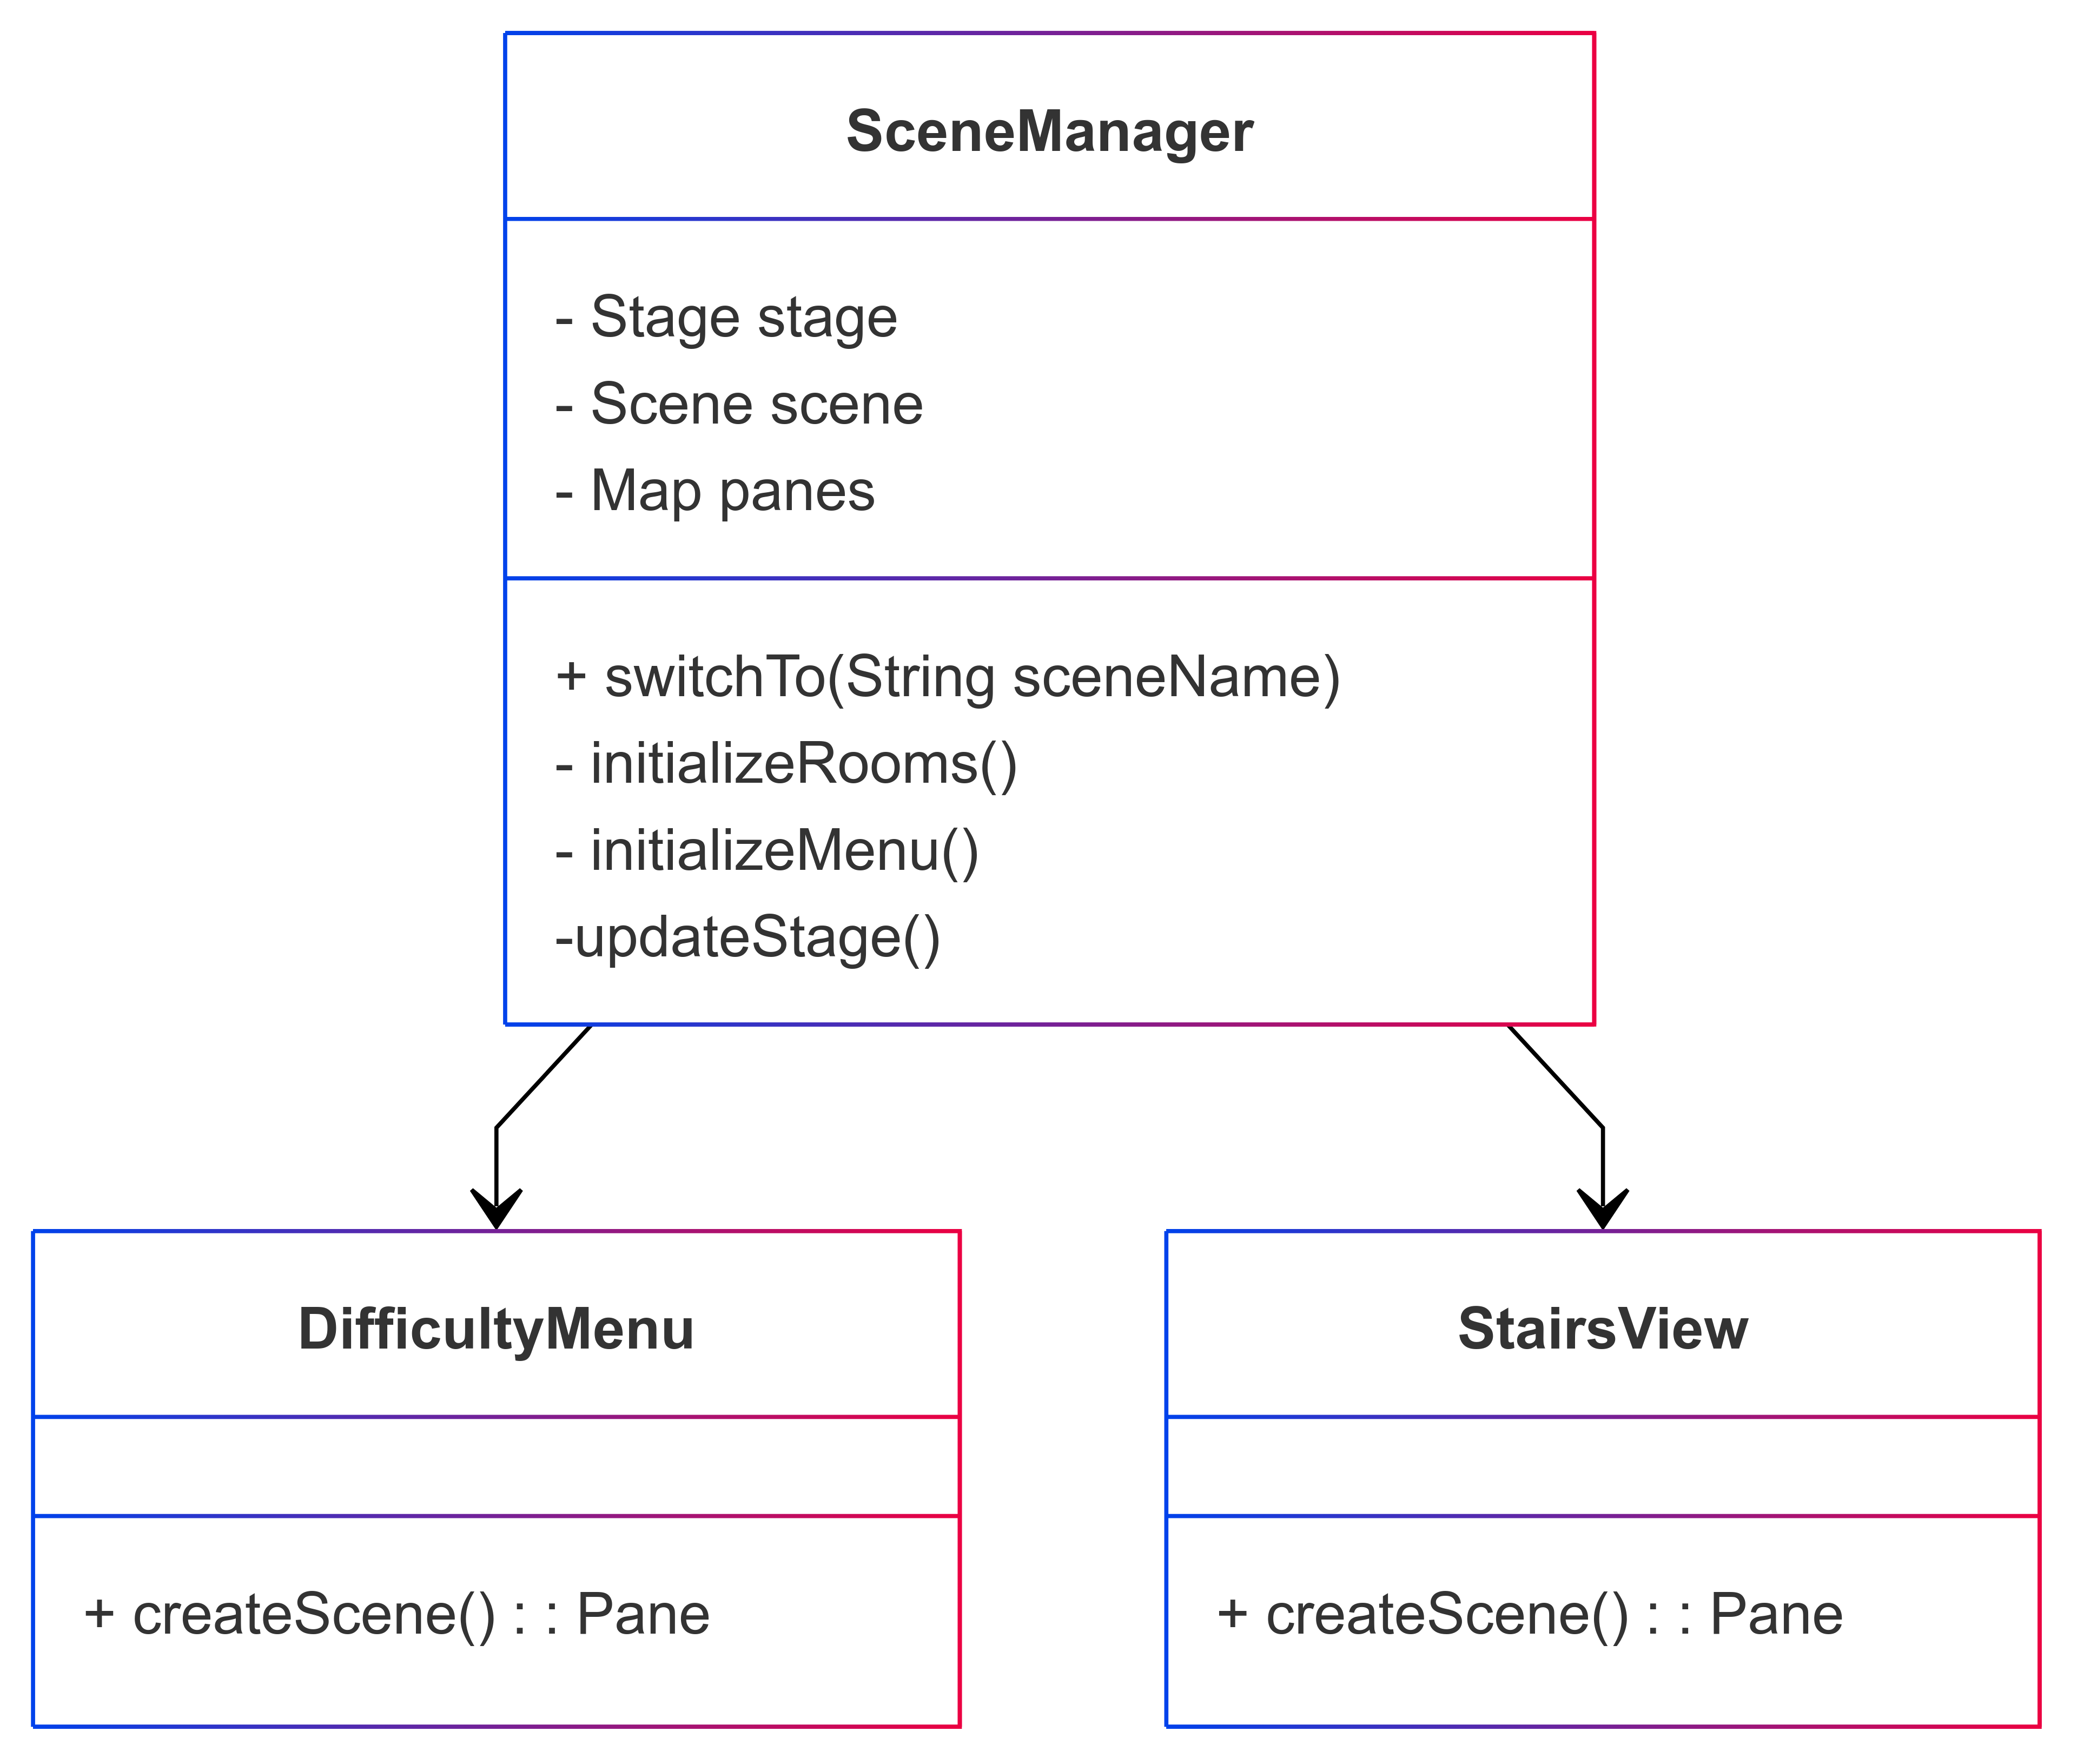
\includegraphics[width=\textwidth]{img/scenemanager.png}
\caption{Rappresentazione UML del pattern Factory per la gestione delle viste (esempio con 2 viste)}
\label{img:factory}
\end{figure}

\paragraph{Problema} Il gioco presenta diverse viste (menu iniziale, viste delle stanze, ecc.) e occorre gestire la visualizzazione in modo coerente.
  
\paragraph{Soluzione} Il sistema utilizza il pattern Factory: le classi che implementano le viste (\texttt{NomevistaView}) vengono registrate nel mapping interno del \texttt{SceneManager}, il quale si occupa di:
\begin{itemize}
	\item Inizializzare le viste relative alle schermate iniziali all'avvio del gioco.
	\item Inizializzare le viste degli elementi di gioco dopo il caricamento della torre.
	\item Caricare e visualizzare il nuovo Pane tramite il metodo \texttt{switchTo}.
\end{itemize}
Questa soluzione consente di passare agevolmente da una vista all'altra, facilitando l'aggiunta di nuove interfacce.

\subsubsection{Stanze del gioco}

\begin{figure}[H]
\centering{}
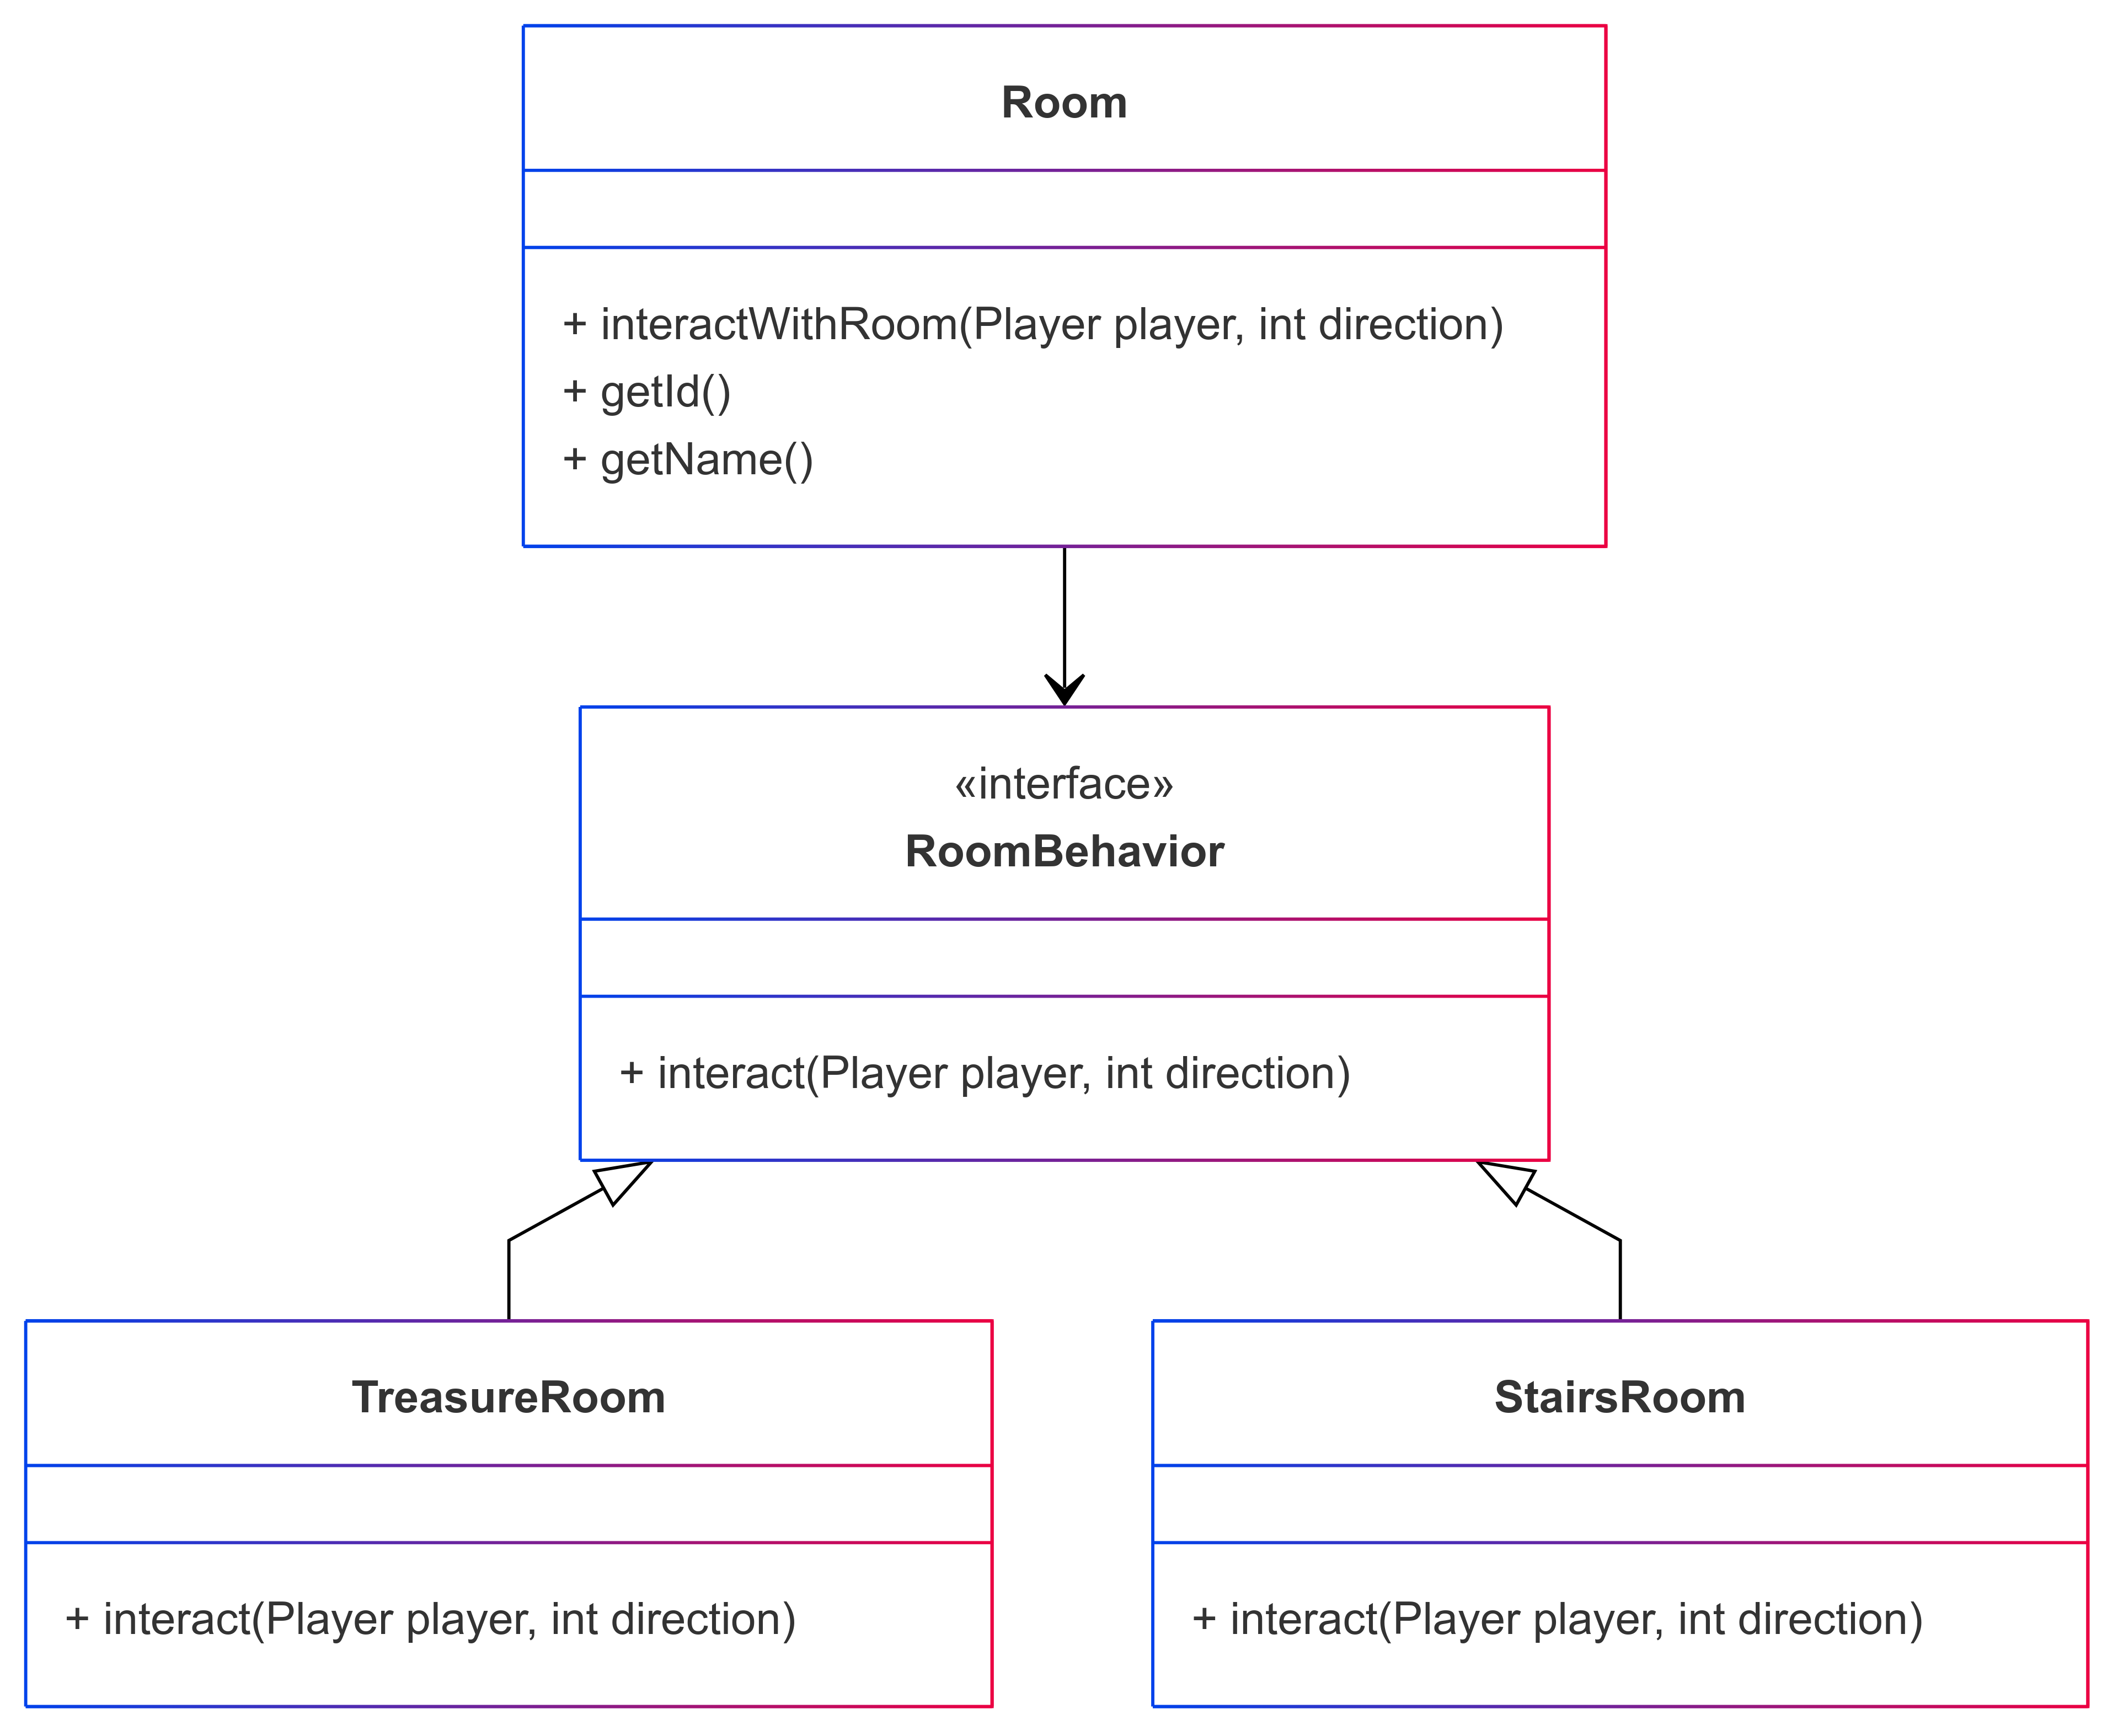
\includegraphics[width=\textwidth]{img/behavior.png}
\caption{Rappresentazione UML del pattern Strategy per le stanze del gioco}
\label{img:rooms}
\end{figure}

\paragraph{Problema} Temple Tower prevede diverse tipologie di stanze, ciascuna con contenuti differenti.
  
\paragraph{Soluzione} Il sistema usa il pattern Strategy per modellare le stanze: le implementazioni di \texttt{RoomBehavior} possono essere facilmente sostituite. Ad esempio, il metodo \texttt{interact()} nella classe \texttt{Trap} sottrarrà punti vita al giocatore, mentre nella stanza \texttt{Stairs} il metodo cambierà il piano.
  
Questo pattern consente di ampliare i tipi di stanze con minime modifiche al codice esistente.

\chapter{Sviluppo}
\section{Testing automatizzato}
Per il testing generale di Temple Tower è stata utilizzata la suite JUnit.
\subsection*{Controller}
Nel controller sono state testate tutte le classi che vi interagiscono, oltre alla view:
\begin{itemize}
 \item Giocatore: vita, cambio stanza e armi.
 \item Nemico: vita e attacchi.
 \item Cambio piano.
 \item Boss finale: sistema di decisione all'arrivo nella stanza del boss.
\end{itemize}

\section{Note di sviluppo}

\subsection{Cobo}
\subsubsection{Uso di parti della libreria JDK non spiegate a lezione}
Uso di \texttt{Clip} per gestire la riproduzione audio \href{https://google.com}{permalink}.
\subsubsection{Uso di librerie di terze parti}
Uso di SLF4J per il logging \href{https://google.com}{permalink}.

\subsection{Vignali}
\subsubsection{Utilizzo della libreria gson}
Utilizzato principalmente in GameDataManager per l'importazione e il caricamento delle torri: \href{https://google.com}{permalink}.
\subsubsection{Utilizzo della libreria JavaFX}
Utilizzato all'interno di ModdingMenuView insieme a codice CSS: \href{https://google.com}{permalink}.
\subsubsection{Utilizzo della libreria SLF4J}
Impiego prevalente per la gestione dei log, sia nei test che nel codice: \href{https://google.com}{permalink}.
\subsubsection{Utilizzo della libreria Apache Commons IO}
Impiegata per la gestione dei file, in combinazione con java.util, durante l'importazione: \href{https://google.com}{permalink}.
\subsubsection{Utilizzo della libreria Java util zip}
Utilizzata per la decompressione dei file: \href{https://google.com}{permalink}. 
\subsubsection{Utilizzo di stream e lambda expressions}
Impiego in diverse parti del codice – esempio: \href{https://google.com}{permalink}.
\subsubsection{Utilizzo di Optional}
Utilizzato in varie parti del codice – esempio: \href{https://google.com}{permalink}.

\subsection{Mularoni}
\subsubsection{Utilizzo di lambda expressions} – Esempio: \href{https://github.com/Matt2309/temple-tower/blob/297b37062035f41c3e9258656beace208905a368/src/main/java/it/unibo/templetower/controller/GameControllerImpl.java#L206}{permalink}.
\subsubsection{Utilizzo di \texttt{Threading e Task} in JavaFX per prevenire race condition} – Esempio: \href{https://github.com/Matt2309/temple-tower/blob/297b37062035f41c3e9258656beace208905a368/src/main/java/it/unibo/templetower/view/MainFloorView.java#L90}{permalink}.
\subsubsection{Utilizzo della libreria SLF4J} – Esempio: \href{https://github.com/Matt2309/temple-tower/blob/297b37062035f41c3e9258656beace208905a368/src/test/java/it/unibo/templetower/ControllerTest.java#L27}{permalink}.
\subsubsection{Cerchi con JavaFX} – Fonte: \href{https://stackoverflow.com/questions/70876114/click-to-draw-a-shape-circle}{Stackoverflow}.
\subsubsection{Immagini con JavaFX} – Fonte: \href{https://stackoverflow.com/questions/52229984/javafx-imageview-actions}{Stackoverflow}.
\subsubsection{Uso di Platform.runLater()} – Fonte: \href{https://stackoverflow.com/questions/13784333/platform-runlater-and-task-in-javafx}{Stackoverflow}.

\subsection{Montanari}
\subsubsection{Uso di SLF4J per il logging}
Il progetto utilizza SLF4J per la gestione dei log, garantendo un monitoraggio efficace degli eventi di gioco.\newline
Esempio:
\begin{verbatim}
private static final Logger LOGGER = LoggerFactory.getLogger(GameControllerImpl.class);
\end{verbatim}
\href{https://github.com/}{Link al codice su GitHub}.

\subsubsection{Uso di Lambda Expressions}
Per gestire gli eventi, il codice utilizza espressioni lambda che migliorano la leggibilità e riducono la verbosità.\newline
Esempio:
\begin{verbatim}
attackBt.setOnAction(e -> this.performAttack());
\end{verbatim}
\href{https://github.com/}{Link al codice su GitHub}.

\subsubsection{Gestione del multithreading con Platform.runLater}
JavaFX richiede che gli aggiornamenti dell'interfaccia avvengano nel thread principale; \texttt{Platform.runLater} garantisce operazioni sicure.\newline
Esempio:
\begin{verbatim}
Platform.runLater(() -> playerHpBar.setProgress(newHealth / (double) maxHealth));
\end{verbatim}
\href{https://github.com/}{Link al codice su GitHub}.

\subsubsection{Utilizzo di Timeline e KeyFrame per le animazioni}
Il codice impiega \texttt{Timeline} e \texttt{KeyFrame} per creare effetti visivi durante attacchi e riduzioni della vita.\newline
Esempio:
\begin{verbatim}
Timeline attackAnimation = new Timeline(
new KeyFrame(Duration.seconds(0.5), e -> enemyHpBar.setProgress(newEnemyHp / (double) maxEnemyHp))
);
attackAnimation.play();
\end{verbatim}
\href{https://github.com/}{Link al codice su GitHub}.

\subsubsection{Utilizzo di JavaFX Scene Graph}
La UI è costruita utilizzando StackPane, HBox, VBox e BorderPane.\newline
\href{https://github.com/}{Link al codice su GitHub}.

\chapter{Commenti finali}

\section{Vignali}

\section{Mularoni}
All'interno del team, mi sono occupato della gestione degli elementi di gioco, nonchè della schermata circolare delle stanze e della vista del boss finale.\newline
Considerando il tempo a disposizione e gli impegni, reputo il progetto "accettabile", sebbene con un grande potenziale inespresso, sia per la scarsa divisibilità del lavoro che per l'organizzazione generale.

\section{Montanari}
Durante lo sviluppo del progetto, mi sono occupato principalmente del sistema di combattimento, della creazione delle varie view di gioco e del controller in modo da far comunicare tutte le classi tra di loro. Ritengo che i miei punti di forza siano stati la capacità di problem-solving, la scrittura di codice efficiente e la collaborazione con il team. Tuttavia, ho riscontrato alcune difficoltà, in particolare nella gestione del tempo e nel debugging di problemi complessi.

\subsubsection{Ruolo all'interno del gruppo}
All'interno del team, il mio ruolo è stato quello di sviluppatore principale per il sistema di combattimento e le interfacce di gioco, oltre a occuparmi della logica di comunicazione tra le classi. Ho contribuito a garantire che tutte le componenti funzionassero correttamente insieme, cercando di mantenere un buon livello di collaborazione con gli altri membri.

\subsubsection{Lavori futuri}
Se il progetto dovesse essere portato avanti, credo che si potrebbe migliorare in diverse direzioni. In particolare, suggerirei di ottimizzare le prestazioni del sistema di combattimento, migliorare l'interfaccia utente e aggiungere nuove funzionalità per rendere il gioco più coinvolgente. Inoltre, potrebbe essere utile impiegare il progetto come base per un gioco più ampio o come portfolio personale per dimostrare le competenze acquisite.

Nel complesso, questa esperienza mi ha permesso di migliorare le mie competenze in programmazione, gestione delle comunicazioni tra classi e sviluppo di interfacce di gioco, e sono soddisfatto dei progressi fatti.

\section{Cobo}
Mi sono occupato della gestione dell’audio e dell’integrazione del sistema musicale nel progetto. Ho implementato il controllo della musica di sottofondo, il sistema di regolazione del volume e la gestione della riproduzione attraverso il pattern Singleton. Inoltre mi sono occupato della gestione delle scene e dell’interfaccia utente, implementando i menu, ad esempio quello delle impostazioni che ha pulsanti per il controllo del volume e per la navigazione tra schermate.

\subsubsection{Punti di forza}
Utilizzo avanzato di Java Sound API per il controllo dell’audio.
Implementazione del pattern Singleton con doppia verifica per garantire efficienza e sicurezza.
Utilizzo di JavaFX per un'interfaccia grafica responsive e dinamica.
Creazione di pulsanti grafici con immagini per un’interfaccia più intuitiva.
Organizzazione chiara del codice, rendendo i menu facilmente estendibili.
\subsubsection{Punti di debolezza}
La gestione del volume potrebbe essere migliorata con un'interfaccia utente più intuitiva.
Alcune transizioni tra scene potrebbero essere più fluide e animate.
L’aspetto visivo del menu potrebbe essere più curato con CSS.
\subsubsection{Lavori futuri}
Se il progetto venisse portato avanti, si potrebbe migliorare il sistema audio offrendo un maggiore controllo e una qualità audio migliore. Inoltre si potrebbe aggiungere un file di configurazione per memorizzare le preferenze dell’utente e un design UI più accattivante con animazioni e transizioni fluide.
Durante il corso mi sono trovato molto bene con i docenti, sia per la chiarezza delle spiegazioni sia per l’efficacia dei metodi di insegnamento adottati. Il materiale fornito e l’approccio didattico hanno reso l’apprendimento strutturato e accessibile, facilitando la comprensione anche di concetti avanzati.

\appendix
\chapter{Guida utente}

L'applicazione è stata progettata per essere intuitiva e di facile utilizzo. Di seguito, una breve guida per iniziare a giocare:

\begin{enumerate}
    \item \textbf{Avvio e Menu Iniziale:}  
    All'avvio, verrà mostrata la schermata iniziale. Cliccare sul pulsante centrale per accedere al menu principale.

    \item \textbf{Importazione della Torre:}
    \begin{itemize}
        \item Dal menu principale, aprire il \textit{Modding Menu} per importare una torre.
        \item È possibile caricare una torre presente nella repository del progetto o scaricarla tramite il seguente link \href{https://google.com}{Tower Download}.
        \item Ricordarsi di cliccare sul tasto Select per selezionare la torre.
    \end{itemize}

    \item \textbf{Inizio della Partita:}
    \begin{itemize}
        \item Dopo aver scelto la torre, premere il pulsante centrale per avviare il gioco.
        \item Si consiglia di impostare la difficoltà su \textit{facile} per facilitare il testing e l'apprendimento delle dinamiche di gioco.
    \end{itemize}

    \item \textbf{Navigazione Durante il Gioco:}
    \begin{itemize}
        \item Utilizzare i pulsanti in basso per muoversi a destra o a sinistra nelle stanze.
        \item Cliccare il pulsante centrale \textit{Enter} per entrare in una stanza.  
              Una volta all'interno, seguire le istruzioni visualizzate per interagire con gli elementi della stanza.
    \end{itemize}
\end{enumerate}

\textbf{Nota:} Assicurarsi che la torre selezionata sia accessibile (basta permesso di lettura) e che l'applicazione abbia il permesso di creare una cartella user.
\chapter{Esercitazioni di laboratorio}

\subsection{mattia.mularoni@studio.unibo.it}

\begin{itemize}
\item Laboratorio 07: \url{https://virtuale.unibo.it/mod/forum/discuss.php?d=177162#p246190}
 \item Laboratorio 08: \url{https://virtuale.unibo.it/mod/forum/discuss.php?d=178723#p247234}
 \item Laboratorio 09: \url{https://virtuale.unibo.it/mod/forum/discuss.php?d=179154#p247924}
 \item Laboratorio 10: \url{https://virtuale.unibo.it/mod/forum/discuss.php?d=180101#p249553}
 \item Laboratorio 04: \url{https://virtuale.unibo.it/mod/forum/discuss.php?d=12345#p123456}
 \item Laboratorio 06: \url{https://virtuale.unibo.it/mod/forum/discuss.php?d=22222#p222222}
 \item Laboratorio 09: \url{https://virtuale.unibo.it/mod/forum/discuss.php?d=99999#p999999}
\end{itemize}

\subsection{davide.vignali4@studio.unibo.it}

\begin{itemize}
 \item Laboratorio 09: \url{https://virtuale.unibo.it/mod/forum/discuss.php?d=179154#p248027}
\end{itemize}

\subsection{nicolas.montanari3@studio.unibo.it}

\begin{itemize}
 \item Laboratorio 09: \url{https://virtuale.unibo.it/mod/forum/discuss.php?d=179154}
 \item Laboratorio 10: \url{https://virtuale.unibo.it/mod/forum/discuss.php?d=180101}
\end{itemize}


\bibliographystyle{alpha}
\bibliography{13-template}

\end{document}
